\section{Digital Libraries}\index{Digital Libraries}
\label{sec:background:digital-libraries}

\subsection{Definitions}
\label{sec:background:digital-libraries:definitions}

The field of \glspl{dl} \index{Digital Libraries} is a multidisciplinary field that comprises
disciplines such as data management, digital curation, document management,
information management, information retrieval and library sciences. Fox et al.
\citep{Fox1995} outline the varying impressions of \glspl{dl} \index{Digital Libraries} from
persons
in different disciplines and adopt a pragmatic approach of embracing the
different definitions. They further acknowledge the metaphor of the traditional
library as empowering and recognise the importance of knowledge systems that
have evolved as a result. Arms \citep[see][chap. 1]{Arms2000}⁠ provides an
informal definition by viewing a \gls{dl} index{Digital Libraries} as a well organised, managed
network-accessible collection of information---with associated services.

%Nice block diagram on link below...
%http://crd-legacy.lbl.gov/~kewu/ps/LBNL-1677E.pdf

In an attempt to overcome the complex nature of \glspl{dl}, Gon\c{c}alves et
al. \citep{Gonccalves2004}⁠ define a \gls{dl}, using formal methods, by
constructively defining a minimal set of components that make up a \gls{dl}. The set-oriented and functional mathematical formal basis of their
approach facilitates the precise definition of each component as functional
compositions.

The European Union co-funded DELOS\index{DELOS} Network of Excellence on \glspl{dl}
working group proposed a reference model and drafted The \gls{dl}
Manifesto with the aim of setting the foundations and identifying concepts
within the universe of \glspl{dl} \index{Digital Libraries} \citep{Candela2007a}. The DELOS \gls{dl} index{Digital Libraries} reference model envisages a \gls{dl} index{Digital Libraries} universe as a complex
framework and tool having no logical, conceptual, physical, temporal or personal
borders or barriers on information. A \gls{dl} index{Digital Libraries} is perceived as an
evolving organisation that comes into existence through a series of development
steps that bring together all the necessary constituents, each corresponding to
three different levels of conceptualisation of the universe of \glspl{dl}
\citep{Candela2007}⁠. The DELOS \gls{dl} index{Digital Libraries} reference model is discussed in
depth in Section~\ref{sec:background:reference-models-frameworks:delos}.

\subsection{Application domains}
\label{sec:background:digital-libraries:application-domains}

The use of \glspl{dl} \index{Digital Libraries} has become widespread mainly due to the significant
technological advances that have been taking place since the 1990s. The advent
of the Internet has particularly influenced this widespread use. There are
various application domains in which \glspl{dl} \index{Digital Libraries} are used and researchers
are continuously coming up with innovative ways of increasing the footprint of
\gls{dl} index{Digital Libraries} usage. 

Academic institutions are increasingly setting up institutional repositories to
facilitate easy access to research output. \glspl{dl} \index{Digital Libraries} play a vital role
by ensuring that intellectual output is collected, managed, preserved and later
accessed efficiently and effectively. Figure~\ref{fig:background:digital-libraries:zm-cbu-repository} is an illustration of
an institutional repository system---a full text open access institution
repository of the Copperbelt
University\footnote{\url{http://dspace.cbu.ac.zm:8080/jspui}}.

\begin{figure}
 %\begin{center}
 \centering
  \framebox[\textwidth]{%
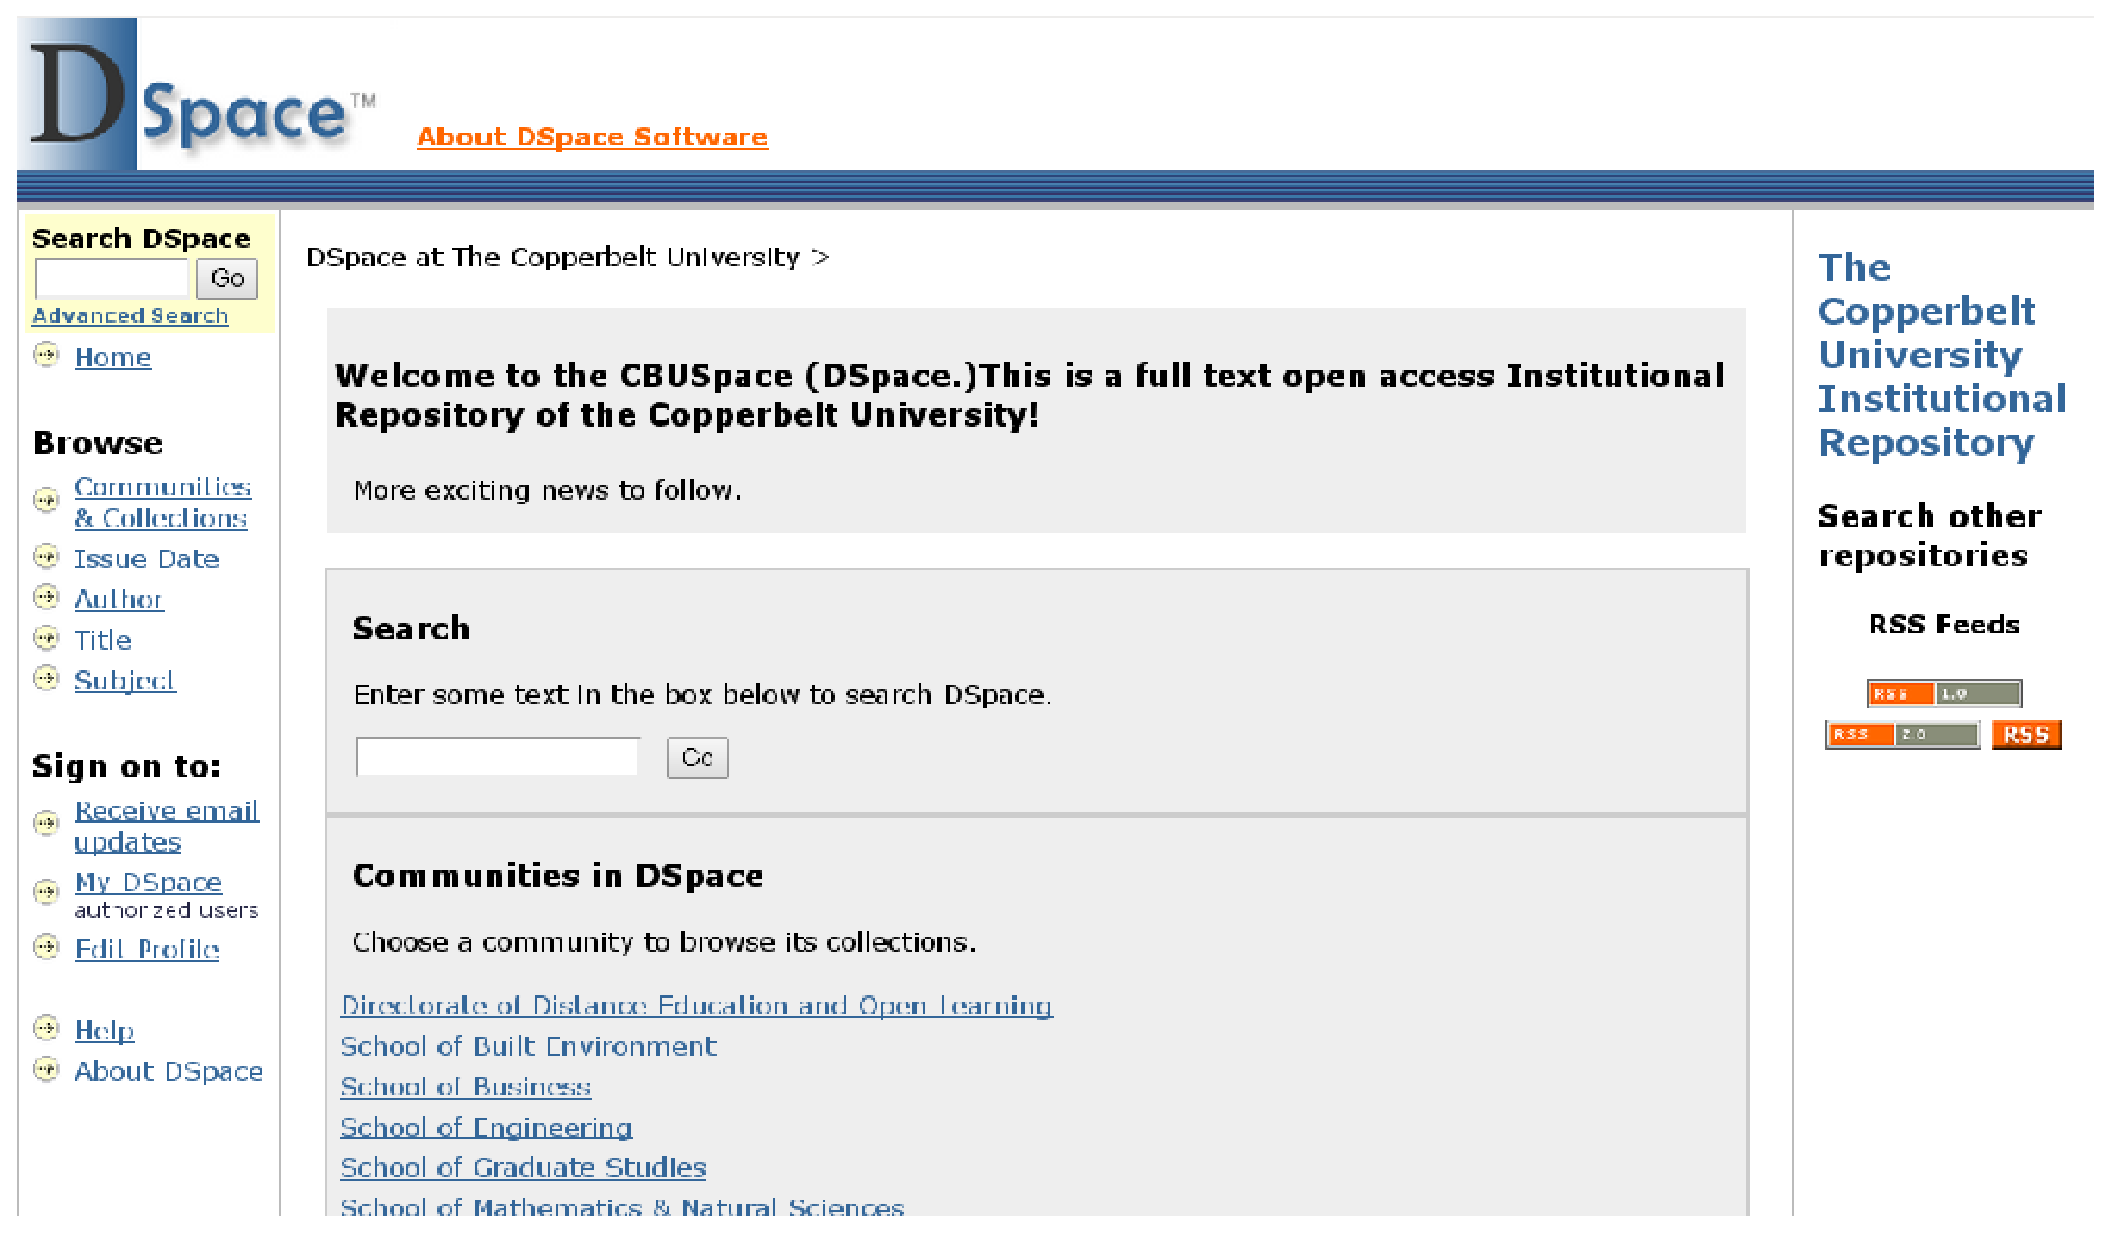
\includegraphics[width=0.95\textwidth]{chapter02/figures/zm-cbu-repository.eps}
  }%
  \caption{Screenshot showing the Copperbelt University institution repository}
  \label{fig:background:digital-libraries:zm-cbu-repository}
 %\end{center}
\end{figure}

Cultural heritage organisations are increasingly digitising historical artifacts
in a quest to display them online to a much wider audience. In light of this,
\glspl{dls} \index{Digital Library System} are being developed to enable easy access to this
information. Figure~\ref{fig:background:digital-libraries:uct-digital-lloydbleekcollection} is a
screen snapshot of the Digital Bleek and Lloyd
Collection\footnote{\url{http://lloydbleekcollection.cs.uct.ac.za}}\index{Bleek\& Lloyd}, which is a
digital collection of historical artifacts that document the culture and
language of the \textbar Xam and !Kun groups of Bushman people of Southern
Africa.

\begin{figure}
 %\begin{center}
  \centering
  \framebox[\textwidth]{%
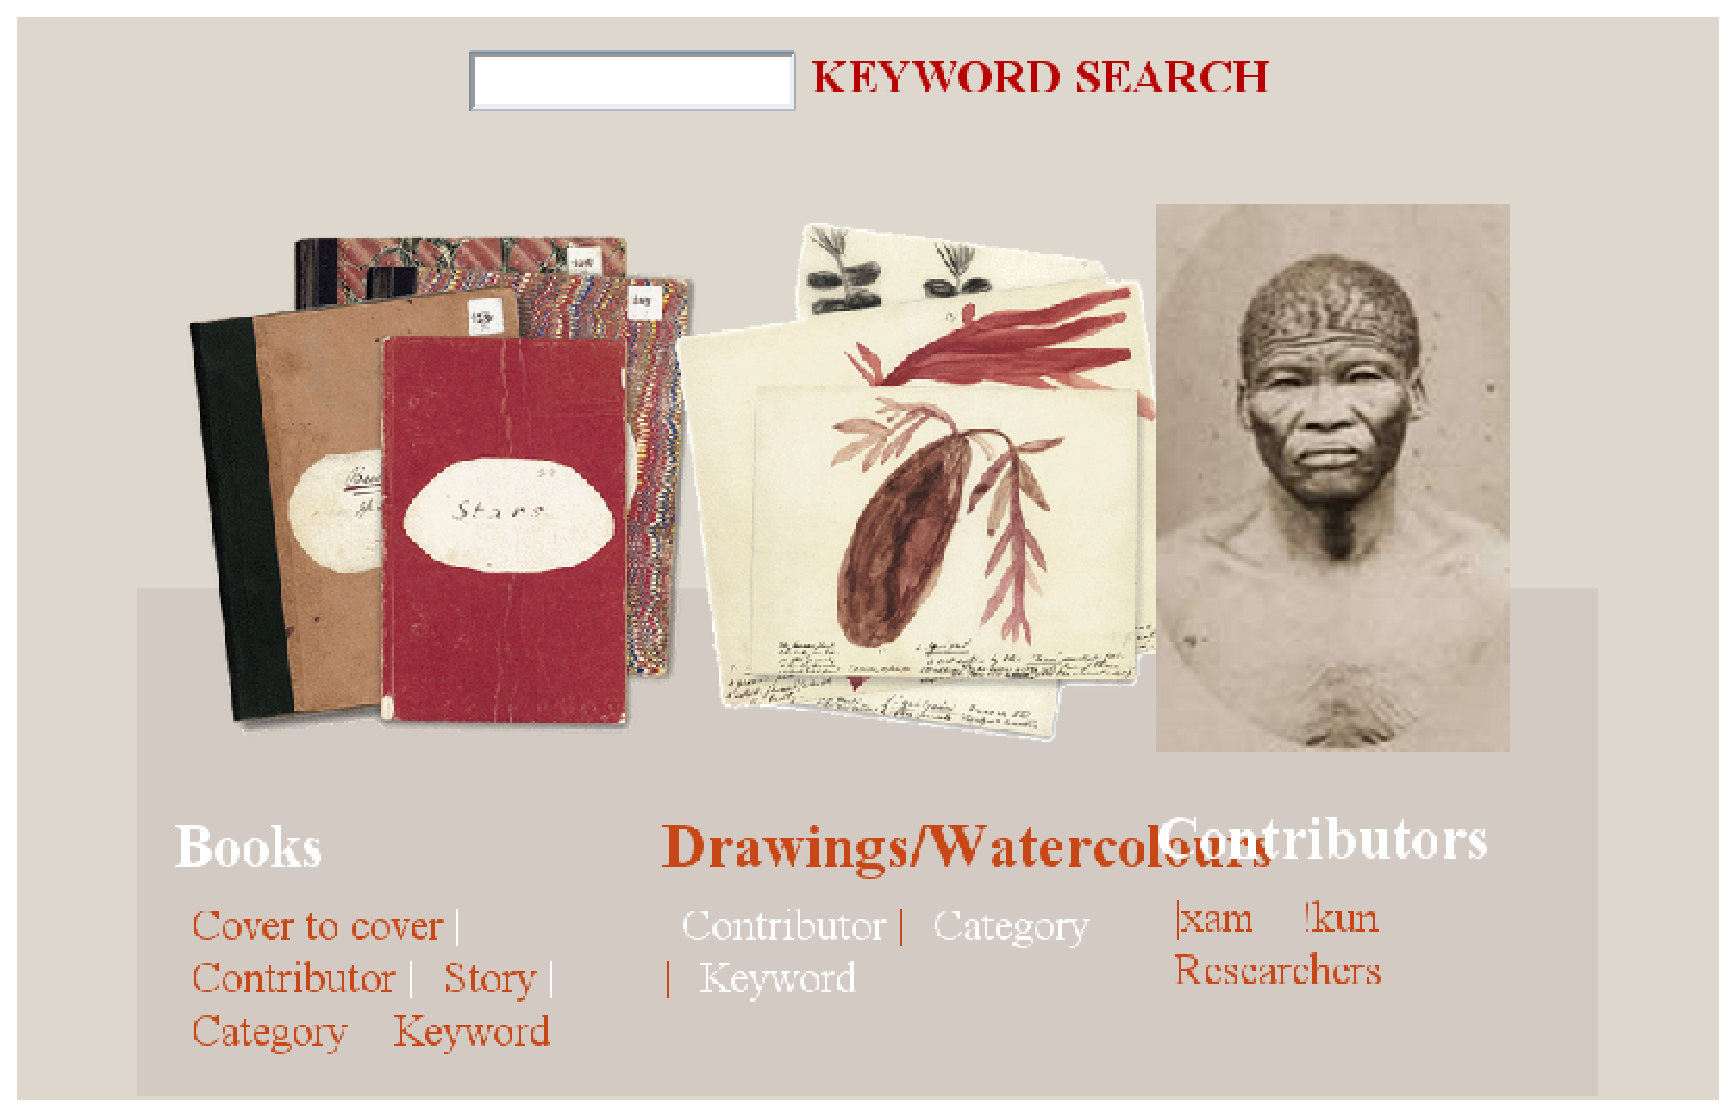
\includegraphics[width=0.95\textwidth]{%
chapter02/figures/uct-digital-lloydbleekcollection.eps}%
}%
\caption{Screenshot showing the digital Bleek\& Lloyd collection}
\label{fig:background:digital-libraries:uct-digital-lloydbleekcollection}
% \end{center}
\end{figure}


There has also been an increasing number of large scale archival projects that
have been initiated to preserve human knowledge and provide free access to vital
information \citep{Hart1992}.

\begin{figure}
 %\begin{center}
 \centering
  \framebox[\textwidth]{%
  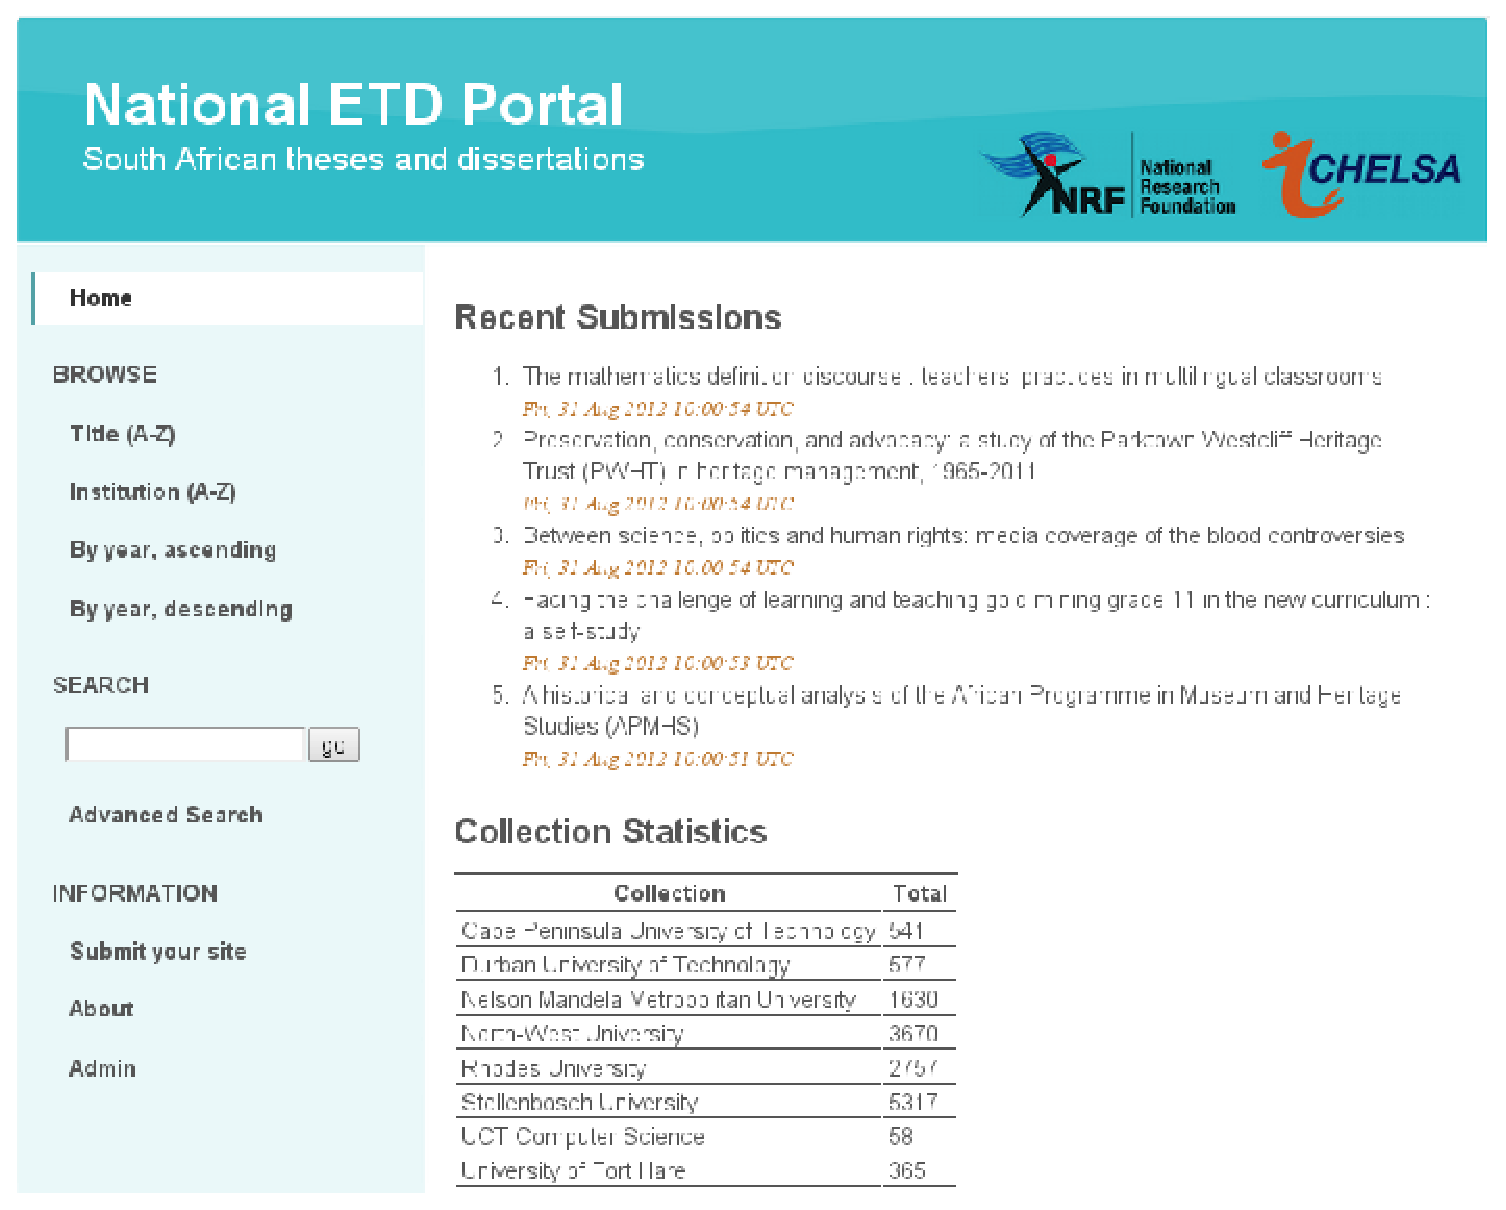
\includegraphics[width=0.95\textwidth]{chapter02/figures/sa-netd-portal.eps}
  }%
  \caption[Screenshot showing the South African NETD portal]{Screenshot showing the South African National Electronic Thesis and Dissertation portal}
  \label{fig:background:digital-libraries:sa-netd-portal}
 %\end{center}

\end{figure}

In addition, a number of federated services are increasingly being implemented
with the aim of making information from heterogeneous services available in
centralised location. Figure~\ref{fig:background:digital-libraries:sa-netd-portal} shows a snapshot of the
South African National Electronic Thesis and Dissertation (NETD) portal\index{NETD}---a federated
service that makes it possible for \glspl{etd}\index{ETD} from various South African universities
to be discovered from a central location.

\begin{figure}
 %\begin{center}
 \centering
  \framebox{%
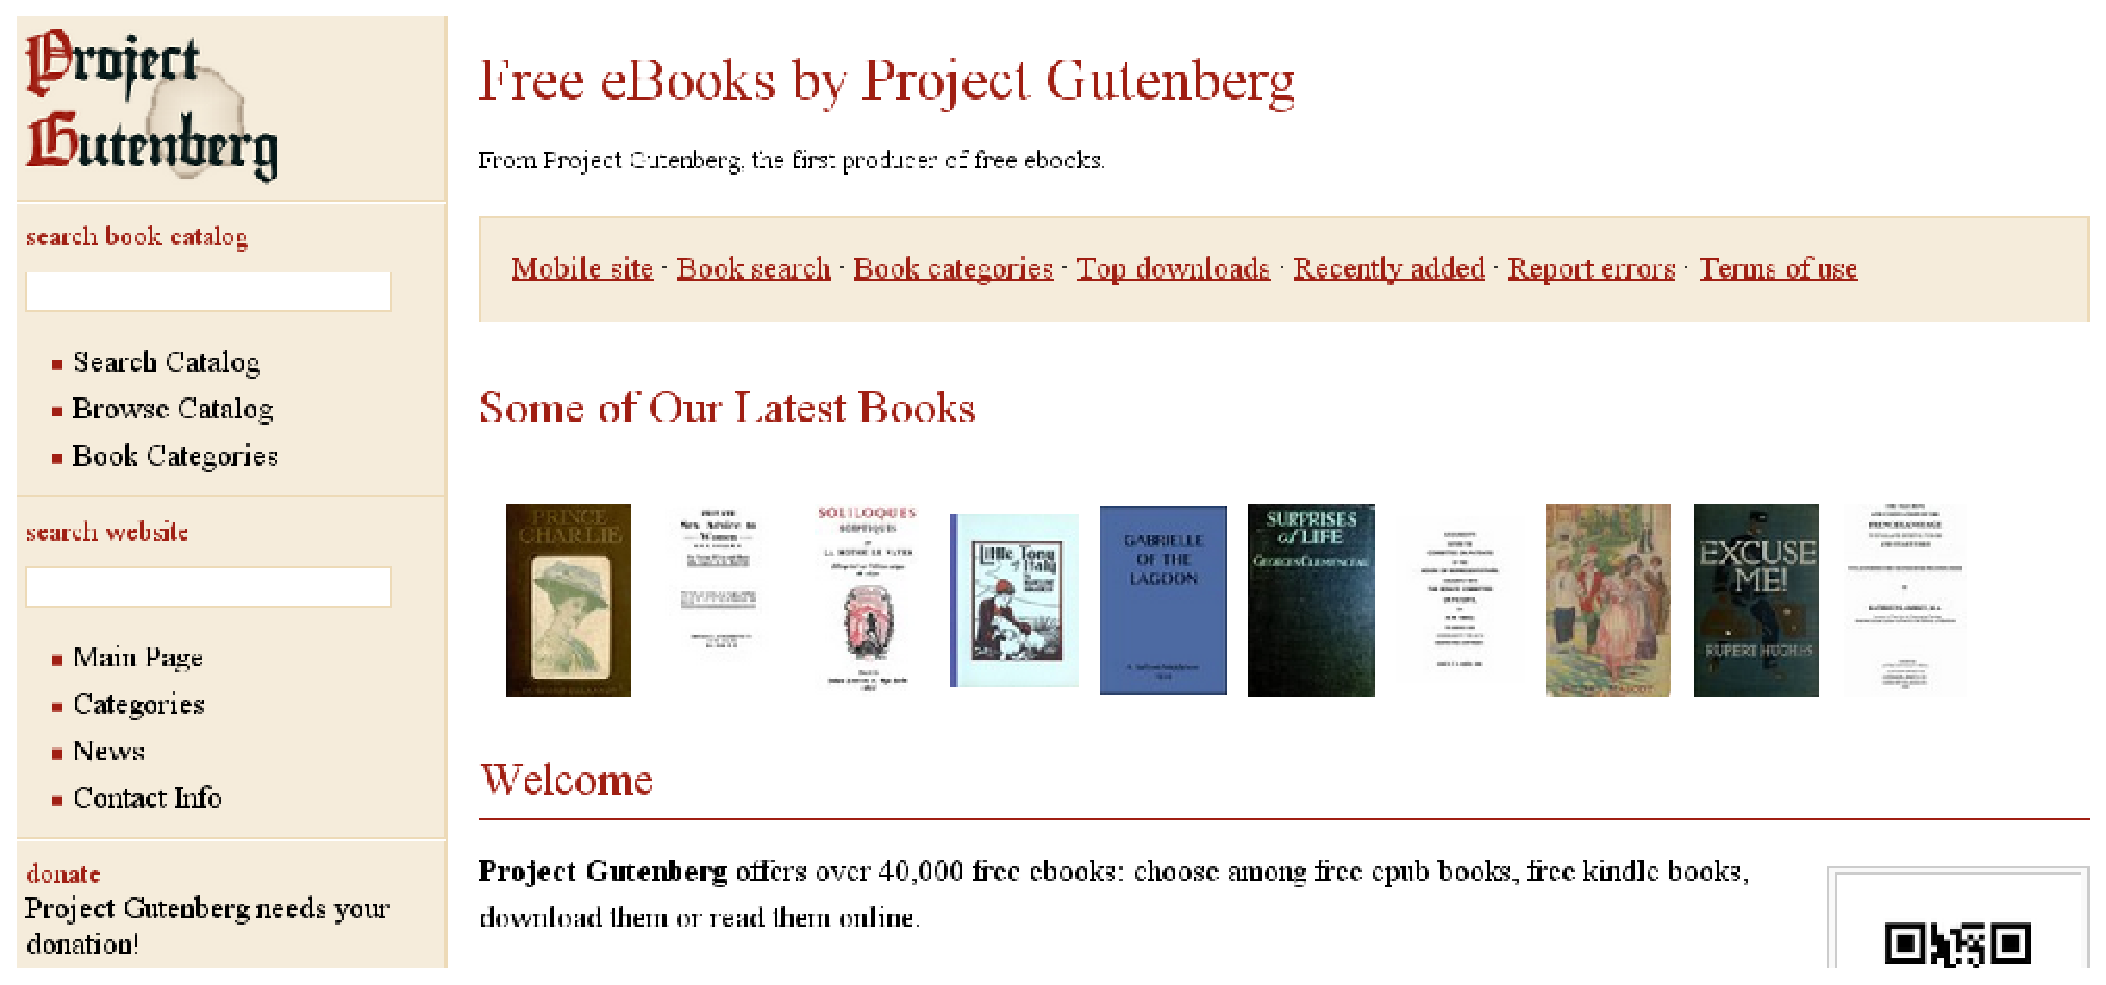
\includegraphics[width=0.95\textwidth]{chapter02/figures/project-gutenberg.eps}
  }%
  \caption{Screenshot showing the Project Gutenburg free ebooks portal}
  \label{fig:background:digital-libraries:project-gutenburg}
 %\end{center}
\end{figure}

\subsection{Summary}
\label{sec:background:digital-libraries:summary}

The massive number of physical copies being digitised, coupled with the increase in the generation of born-digital objects, has created a need for tools and services---\glspl{dl}---for making these objects easily accessible and preservable over long periods of time. The importance of these systems is manifested through their ubiquitous use in varying application domains.

This section broadly defined and described \glspl{dl}, and subsequently discussed some prominent application domains within which are currently used.